\documentclass{beamer}
\usetheme{Darmstadt}
\usepackage{comment}
\usepackage[utf8]{inputenc}    % Para escribir acentos y caracteres especiales
\usepackage{graphicx}          % Para insertar imágenes
\usepackage{booktabs}          % Para tablas más bonitas
\usepackage{enumitem}
\usepackage{amsmath}           % Para escribir ecuaciones
\usepackage{tikz}              % Para gráficos vectoriales
\usetikzlibrary{calc}          % Para coordenadas calculadas con TikZ
\usepackage{pgfplots}          % Para gráficos matemáticos
\pgfplotsset{compat=1.18}      % Evita errores por compatibilidad

\title{Ayudantía 1 \\ Bonos \\ \large\textit{Instrumentos Derivados}}
\author{
  \texorpdfstring{
    \textbf{Profesor:} Francisco Rantul \\[0.3em]
    \textbf{Ayudante:} Mateo Canales
  }{Profesor: Francisco Rantul, Ayudante: Mateo Canales}
}
\subject{Instrumentos Derivados}
\institute{Universidad Diego Portales}
\date{31 De Marzo, 2025}

\begin{document}

% Portada
\begin{frame}
    \titlepage
    \vfill
    \centering
    \includegraphics[width=2.3118cm]{../imagenes/logo.png}
  \end{frame}
\begin{frame}
  \frametitle{Contenido}
  \tableofcontents
\end{frame}
\begin{frame}
  \frametitle{Caso}

  Los precios de los pagarés descontables del Banco Central de Chile (PDBC)
  a 6 meses y a 1 año son de \$94 y \$89 respectivamente. 
  
  Un bono del Banco Central de Chile en pesos (BCP) a 1,5 años que paga cupón de 
  \$4 cada 6 meses tiene un precio de \$94{,}84. Un BCP a 2 años que paga
  cupón de \$5 cada 6 meses tiene un precio de \$97{,}12.

\end{frame}
\section{Preguntas}
  \begin{frame} 
  
\begin{enumerate}[label=\textbf{\alph*)}]
  \item Calcule la curva cero de 6 meses, 1 año, 1,5 años y 2 años.
   Utilice capitalización continua.
  
  \item Grafique la curva cero y comente (sin realizar cálculos) si 
  la pendiente de la curva de los bonos del BCCh (con cupones) es 
  positiva o negativa. ¿Qué factor explica el \textit{spread} entre 
  ambas curvas?, ¿por qué el \textit{spread} aumenta a mayor madurez?
  
  \item Comente cuál es la interpretación económica detrás de la 
  pendiente observada en la curva cero. ¿Qué nos dice respecto a 
  la probabilidad de recesión?
  
  \item Considerando que usted tiene la información de la curva cero, 
  la curva \textit{forward} y la curva de las \textit{yields} de los 
  bonos de gobierno. Señale qué curva usaría para calcular el valor 
  presente de las ganancias o pérdidas de los contratos \textit{forward}.
  
  \item ¿Cuál es el rol de las probabilidades neutrales al riesgo en d)?, 
  ¿qué rol juega la condición de no arbitraje?
  
  \item Calcule el punto a) utilizando matrices en Excel/R/Phyton.
\end{enumerate}

  \end{frame}  

%Pregunta a parte 1
\begin{frame}

    \frametitle{Pregunta a$)$ parte 1}
    \LARGE {\underbar{Calcule la curva cero de 6 meses}}\\[1em]
    Datos: \footnotesize {Tiempo = 6 meses; Tasa = Desconocida; Precio futuro = \$94}
    \footnote{\textbf{Fórmula a utilizar:} Capitalización contínua
    \textcolor{blue}{$F = P \cdot e^{-rt}$}}

\end{frame}
% Gráfico Sin(x)
\begin{frame}
  \frametitle{Gráfico PGFPlots}
  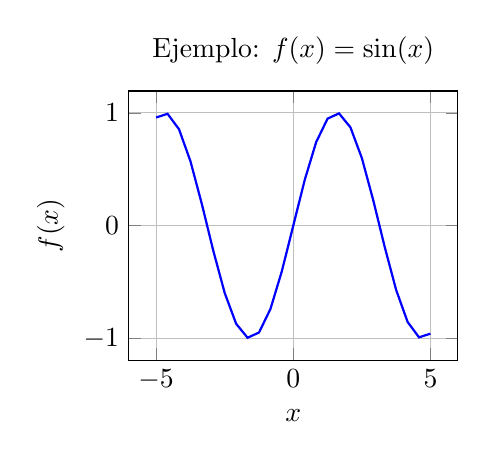
\begin{tikzpicture}
    \begin{axis}[
        width=6.5cm, scale=0.85, clip=true,
        xlabel={$x$},
        ylabel={$f(x)$},
        title={Ejemplo: $f(x)=\sin(x)$},
        grid=major,
        ]
        \addplot[blue, thick] {sin(deg(x))};
    \end{axis}
  \end{tikzpicture}
  \end{frame}
\section{Ejercicios}
\begin{frame}
    \centering
    \Huge \insertsection
\end{frame}
\begin{frame}
  \frametitle{Ejercicio 1 A$)$}
  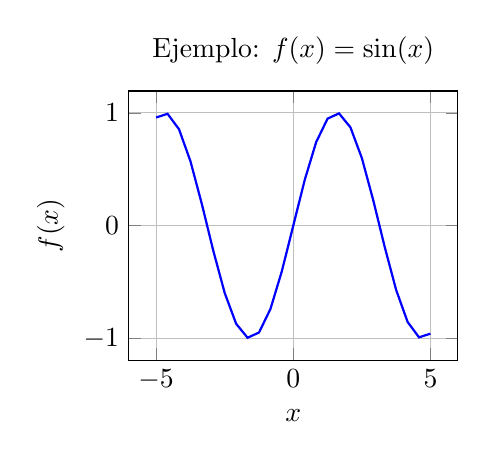
\begin{tikzpicture}
    \begin{axis}[
        width=6.5cm, scale=0.85, clip=true,
        xlabel={$x$},
        ylabel={$f(x)$},
        title={Ejemplo: $f(x)=\sin(x)$},
        grid=major,
        ]
        \addplot[blue, thick] {sin(deg(x))};
    \end{axis}
  \end{tikzpicture}
  \end{frame}
\end{document}